
% ================= ARES USE CASE =================

Sounding rockets provide cost-effective platforms
for scientific research, experimental payload testing,
and the validation of emerging aerospace technologies.
NASA employs suborbital vehicles to evaluate
experimental hardware in flight environments that
cannot be fully replicated on the ground. Such testing
can also support the maturation of technologies
intended for future exploration programs, including
Artemis \cite{NASA_Suborbital,NASA_Artemis_Testing}.

The \ares{} launch vehicle applies these principles
on a student-developed scale, providing a reusable
flight platform for experimental communications,
avionics, and recovery technologies.

\begin{figure}[H]
    \centering
    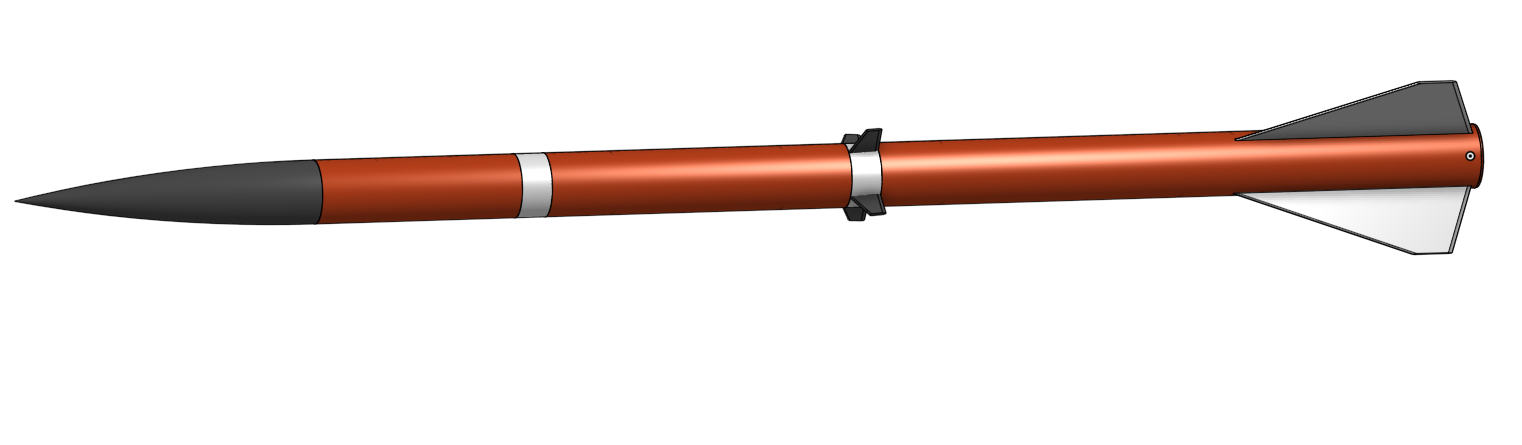
\includegraphics[width=1\linewidth]{Documentation/ARES/Use_Cases/Pics/ARES_CAD.png}
    \caption{\ares rocket CAD model. The rocket will be ~\RHeight ft tall and contain several subsystems, including an automated roll control system. }
    \label{fig:ARES_CAD}
\end{figure}